\documentclass[a4paper]{article}

\usepackage[english]{babel}
\usepackage[utf8]{inputenc}
\usepackage{amsmath}
\usepackage{graphicx}
\usepackage[colorinlistoftodos]{todonotes}
\usepackage{float}

\title{Analysis of 3-fold Cross Validation for KNN, K-means and Hierarchical Clustering implementations}

\author{Saketh Saxena}

\date{\today}

\begin{document}
\maketitle

\section{Introduction}
\label{sec:introduction}
As part of the CS256 Homework 3 I have implemented KNN algorithm, K-means and Hierarchical Clustering (single linkage clustering) for image data, and tested/validated them on images.

\section{3-fold cross validation for KNN}
3 fold cross validation for K nearest neighbour algorithm was done on the dataset, with tunable k value. For my experiments, I have plugged in k = 3 and also computed the accuracies for k = 1 to 10, the results are as depicted in the graphs and screenshot below
\begin{figure}[H]
  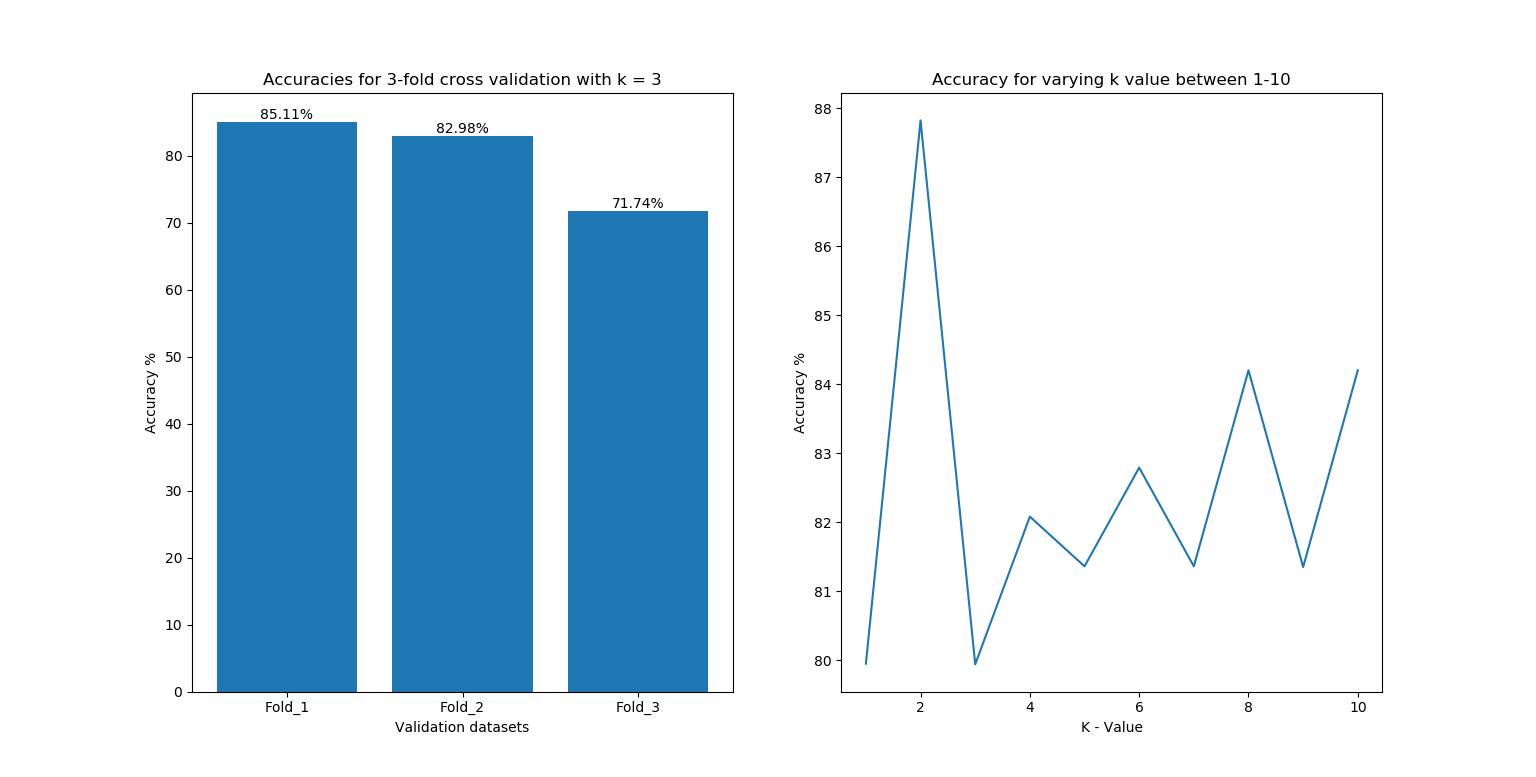
\includegraphics[width=\linewidth]{knn_cross.png}
  \caption{ Bar graph showing accuracy for each fold when k =3 and line plot showing the variation of accuracy for k = 1 to 10 }
  \label{fig:Result 2}
\end{figure}
\begin{figure}[H]
  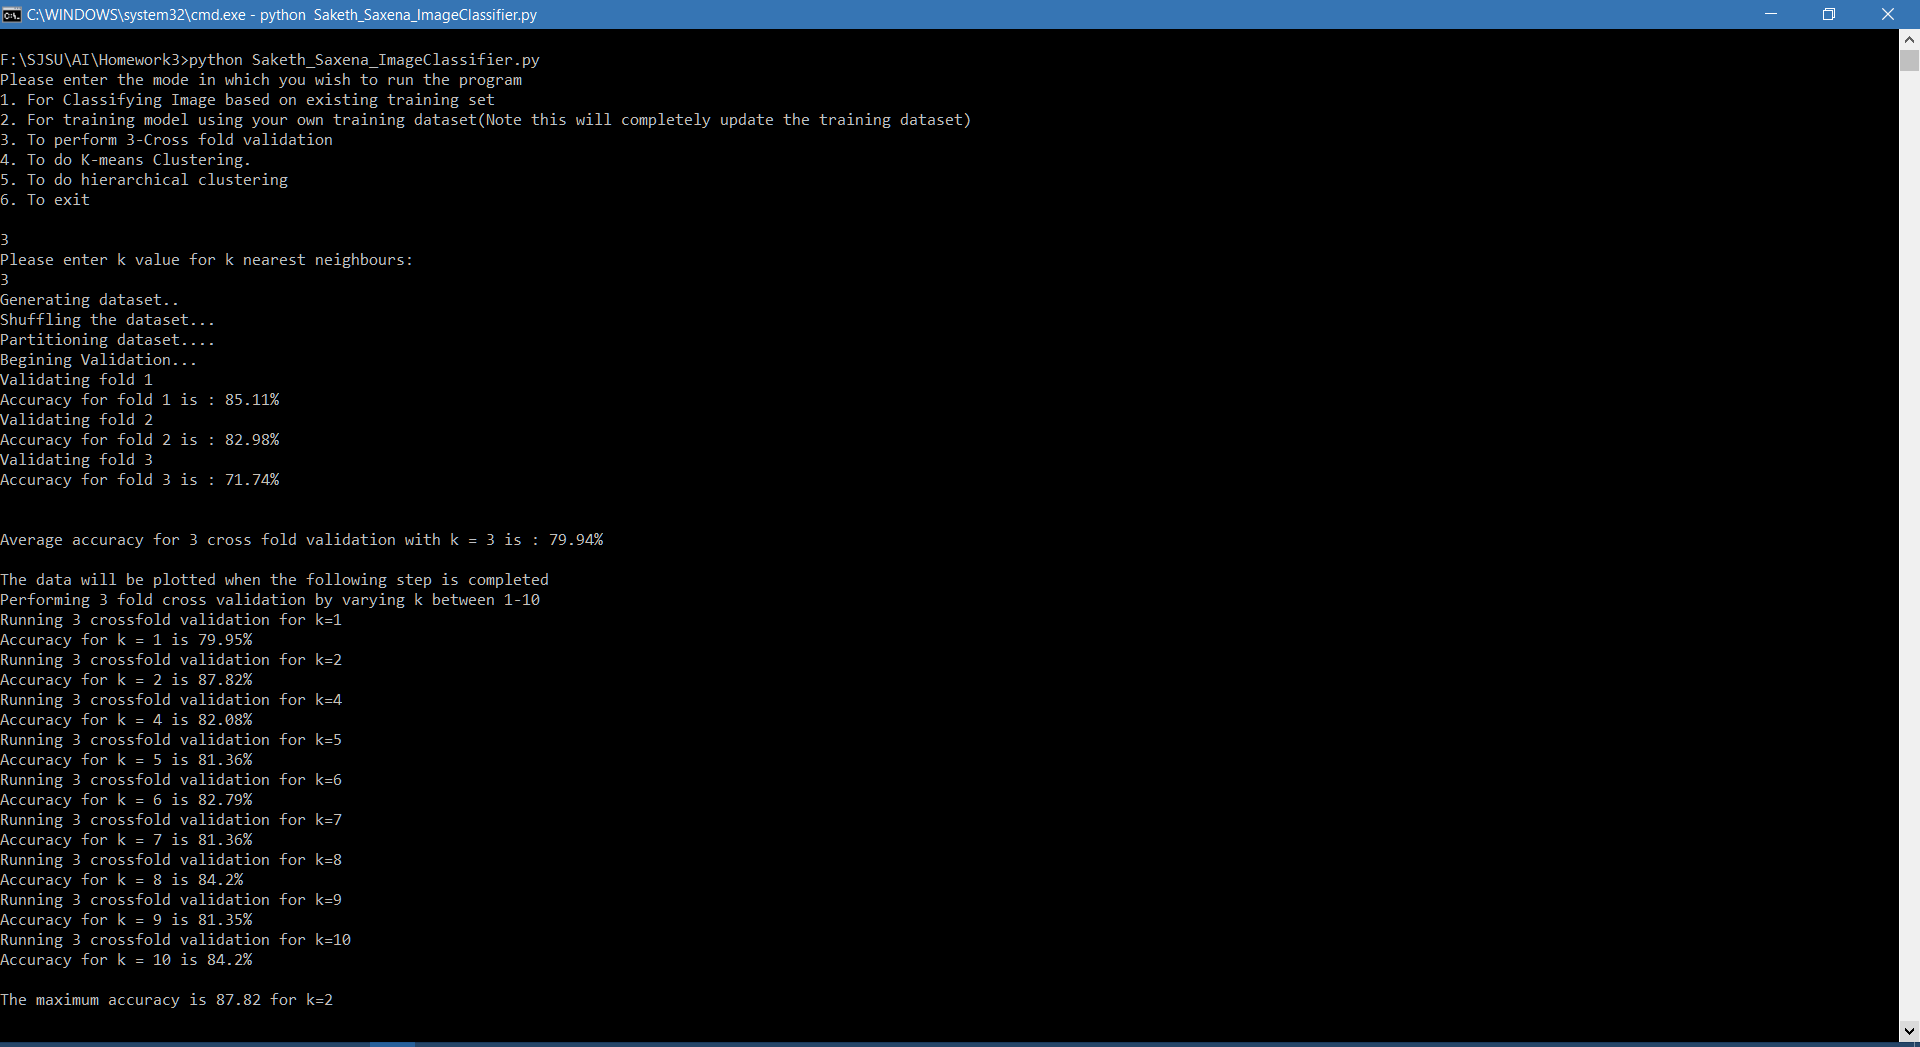
\includegraphics[width=\linewidth]{knn_screenshot_cross.PNG}
  \caption{ Screenshot depicting the output when k=3 }
  \label{fig:Result 3}
\end{figure}



\section{k-means Clustering Algorithm}
The K-means implementation was used to cluster about 140 images belonging to two classes - landscapes(77 in number) and headshots(63 in number).
The implementation was tested with k = 2; and the percentage accuracy for each cluster i.e. number of correctly clustered images upon number of images in the cluster and the average percentage accuracy were computed, the results of which are displayed below:
\begin{figure}[H]
  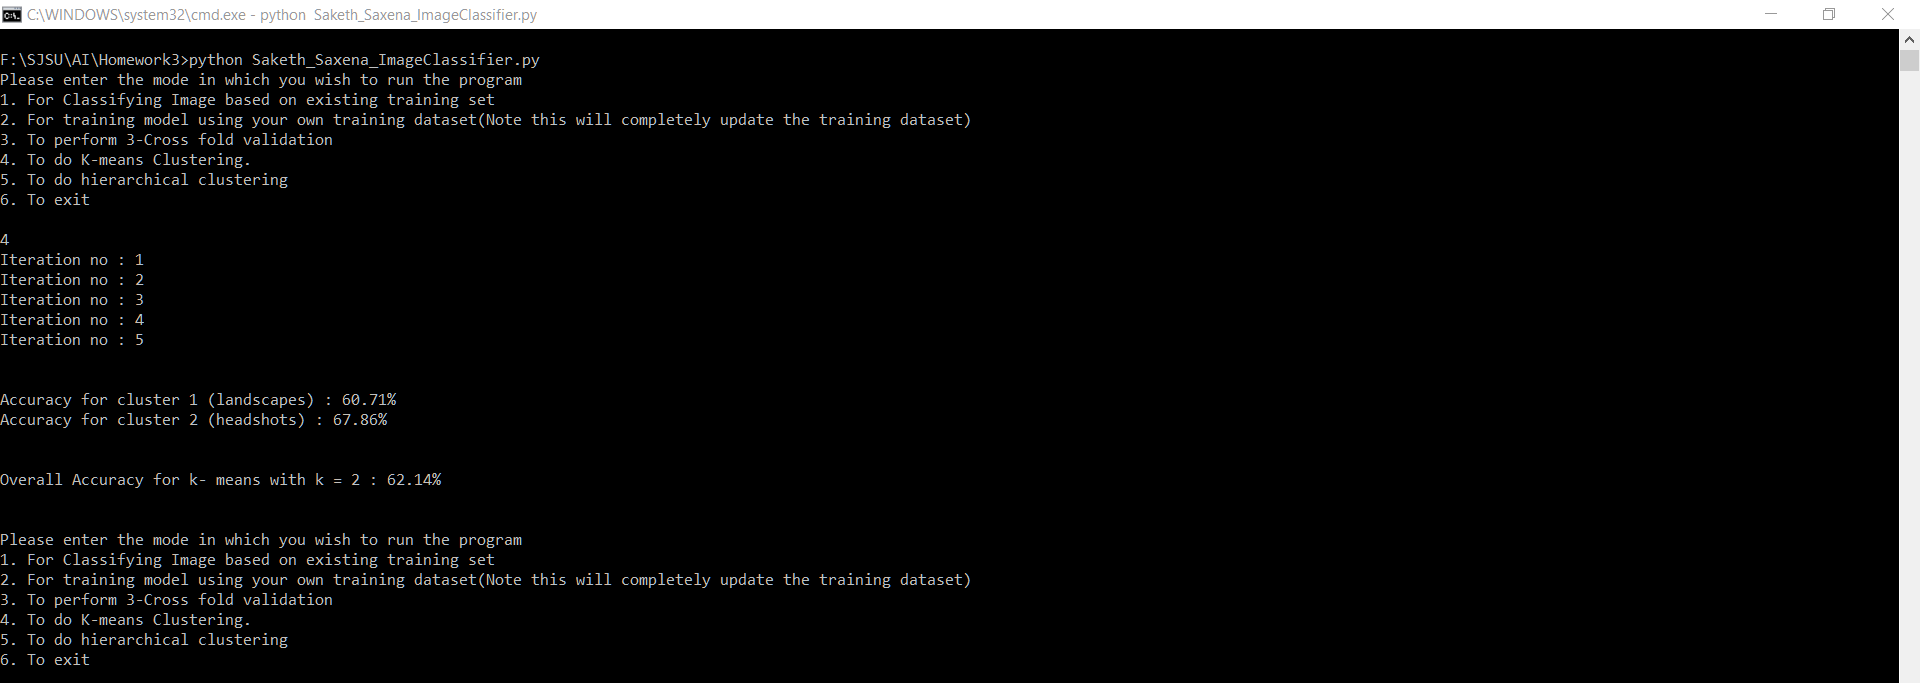
\includegraphics[width=\linewidth]{k_means_result.PNG}
  \caption{Accuracy of C1 = 60.71 \% and C2 = 67.86 \% and Average Accuracy = 62.14\% }
  \label{fig:Result 1}
\end{figure}


\section{Hierarchical/Single linkage Clustering}
The result of the Hierarchical cluster was partitioned into two clusters and the images displayed in the web browser.
The resulting clusters were extremely skewed with cluster being large and one having 1-2 images in them, this could possibly be due to outliers or noise in the data, where some images are extremely different than others.

The implementation was used to cluster 1. landscape and headshot image data 2. 206 images of flags of nations.

\subsection{Clusters for Landscape Vs Headshot}
\begin{figure}[H]
\centering
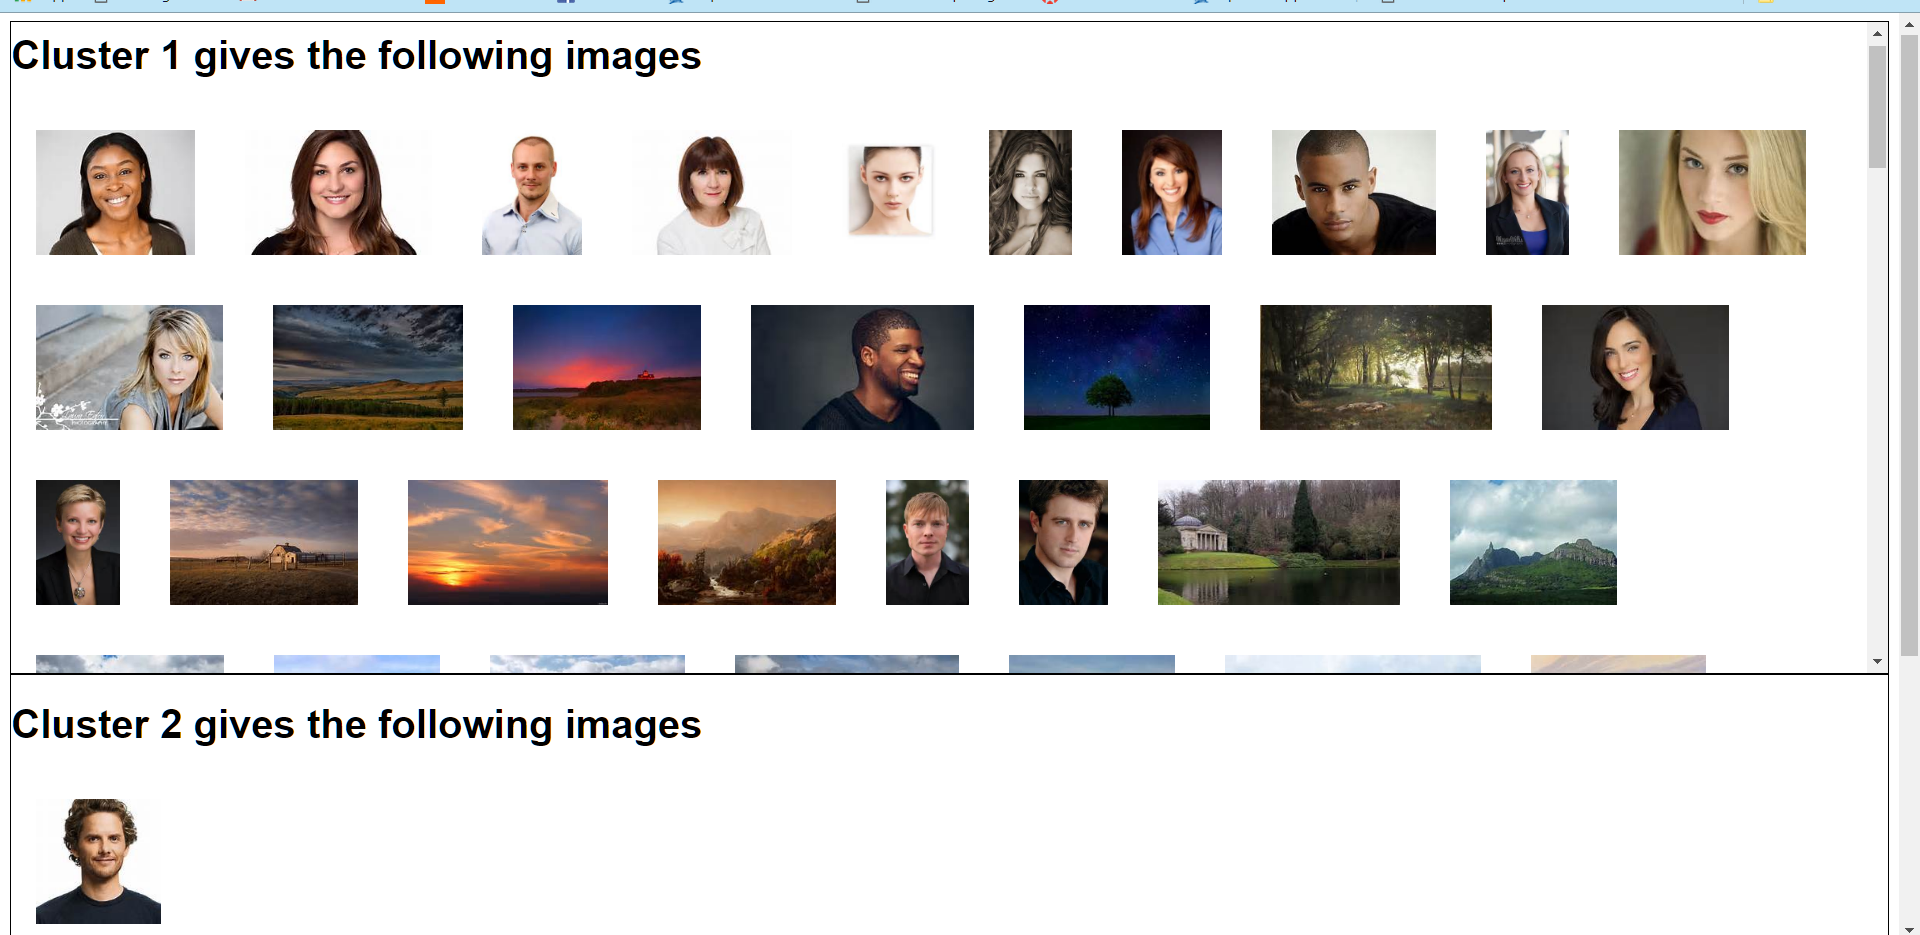
\includegraphics[width=1\textwidth]{head_land.PNG}
\caption{Screenshot of output showing images of headshots vs landscapes in 2 clusters}\label{}
\end{figure}

\subsection{Clusters for flags}
\begin{figure}[H]
\centering
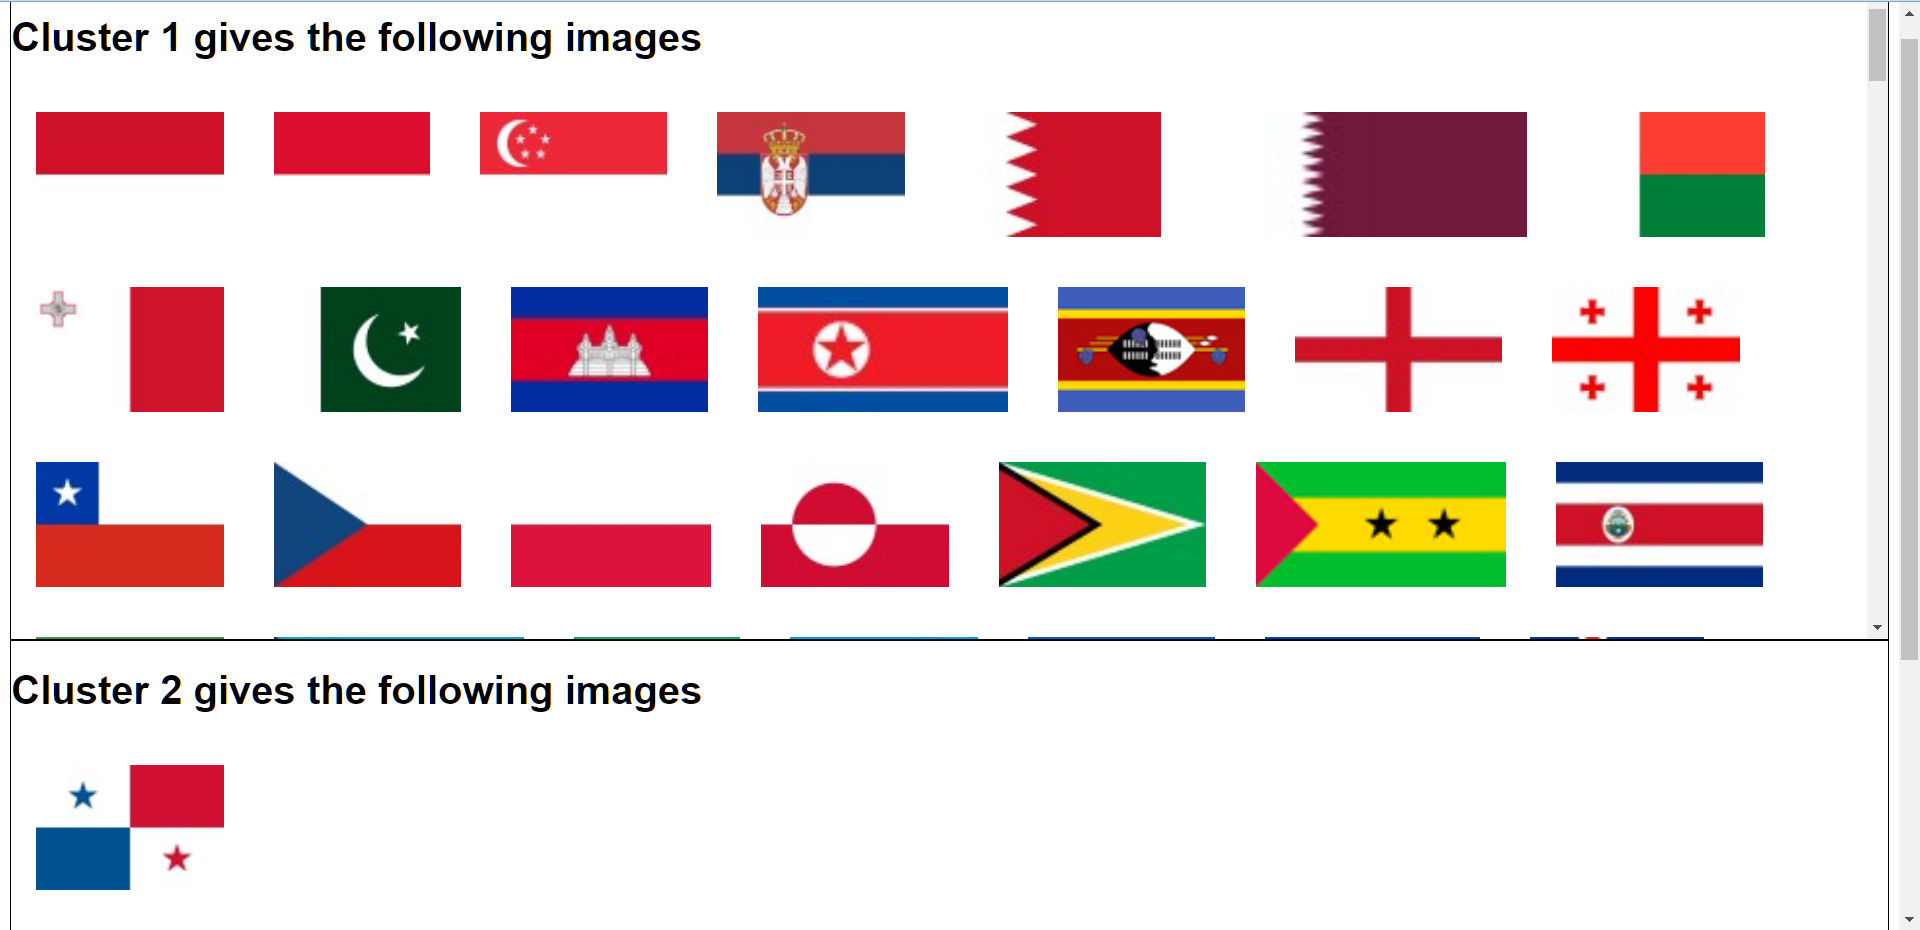
\includegraphics[width=1\textwidth]{flags.PNG}
\caption{Screenshot of output showing images of flags in 2 clusters}\label{
}
\end{figure}
\subsection{Inference of results}
From the results obtained by hierarchical clustering, it shows that this approach is not a very good approach to cluster these datasets, also hierarchical clustering is not particularly effective when the clusters need to be partitioned. 

\end{document}


